\begin{frame}{Structure-Preserving Publicly Verifiable Encryption}
  \begin{block}{Framework}
    \begin{itemize}
    \item $\Setup(\lambda) \to \PPP$
    \item $\KeyGen(\PPP) \to (\PK, \SK)$
    \item $\Enc(\PPP, \PK, m) \to c$
    \item $\Dec(\PPP, \SK, c) \to m \mbox{ or } \bot$
    \item $\Verif(\PPP, \PK, c) \to \{\True, \False\}$
    \end{itemize}
  \end{block}

  \begin{block}{Some parameters}
    
    \begin{itemize}
    \item $\SK = (x_1, x_2)$.
    \item $\PK = (g_1, g_2, X = g_1^{x_1}g_2^{x_2}, \PPP_{SPC}, \vec{\ck}, \PPP_{ABOProof})$.
    \end{itemize}
    where $(g_1, g_2) \in \G^2$ and $(x_1, x_2) \in \mathbb{Z}_p^2$.
  \end{block}
  
\end{frame}

\begin{frame}{Structure-Preserving Publicly Verifiable Encryption}
  \begin{block}{Details of the Encryption algorithm}
    
    \begin{itemize}
    \item Generate $\vec{C} = (C_0, C_1, C_2) = (MX^{\theta}, g_1^{\theta},  g_2^{\theta})$.
    \item $\Sig.\KeyGen(\PPP) \to (\SSK, \SVK)$.
    \item $\Com(\ck, \SVK) \to (\com, \open)$.
    \item $\Prove(\PPP_{ABOProof}, x = (C_1, C_2), w = \theta, tag = \com) \to \pi$ of the fact $\exists \chi$ such that $(C_1, C_2) = (g_1^\chi, g_2^\chi)$.
    \item $\Sig.\Sig(\SSK,(\vec{C},\pi)) \to \sigma$.
    \item Output the ciphertext $(\vec{C}, \pi, \SVK, \com, \open, \sigma) \in \G^{16} \times \hat{\G}^{11}$.
    \end{itemize}

  \end{block}
\end{frame}


\begin{frame}{Proof intuitions}
  \begin{columns}
    \begin{column}{0.5\textwidth}
        \tiny
      \begin{figure}
        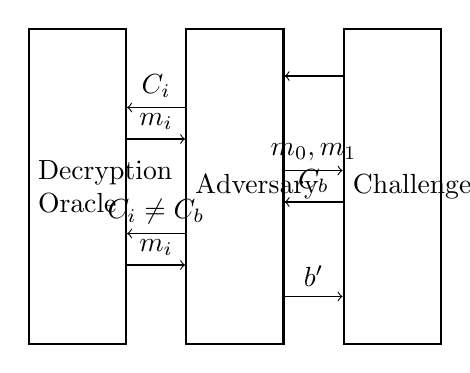
\begin{tikzpicture}
      \node(A)[draw, thick, text width = 1cm, minimum height = 4cm] at (0,0) {Adversary};
      \node(C)[draw, thick, text width = 1cm, minimum height = 4cm] at (2,0) {Challenger};
      \node(D)[draw, thick, text width = 1cm, minimum height = 4cm] at (-2,0) {Decryption Oracle};
      
      \path([yshift = 1.4cm]A.east) edge[<-] node[above]{$\PK$} ([yshift = 1.4cm]C.west);
      \path([yshift = 1cm]D.east) edge[<-] node[above]{$C_i$} ([yshift = 1cm]A.west);
      \path([yshift = 0.6cm]D.east) edge[->] node[above]{$m_i$} ([yshift = 0.6cm]A.west);
      \path([yshift = 0.2cm]A.east) edge[->] node[above]{$m_0, m_1$} ([yshift = 0.2cm]C.west);
      
      \path([yshift = -0.2cm]A.east) edge[<-] node[above]{$C_b$}([yshift = -0.2cm]C.west);
      \path([yshift = -0.6cm]D.east) edge[<-] node[above]{$C_i \neq C_b$} ([yshift = -0.6cm]A.west);
      \path([yshift = -1cm]D.east) edge[->] node[above]{$m_i$} ([yshift = -1cm]A.west);
      
      \path([yshift = -1.4cm]A.east) edge[->] node[above]{$b'$}([yshift = -1.4cm]C.west);
    \end{tikzpicture}
  \end{figure}
    \end{column}

    \begin{column}{0.5\textwidth}

      
      \tiny
      \visible<3->{{\color{red}In SetupABO, $tag^* = \com^*$}}

      Encryption
    \begin{itemize}
    \item Generate $\vec{C}^* = (C_0^*, C_1^*, C_2^*) = (\alt<4->{{\color{red}M_bC_1^{x_1}C_2^{x_2}}}{ M_bX^{\theta^*}}, g_1^{\alt<5->{{\color{red}\theta_1}}{\theta^*}},  g_2^{\alt<5->{{\color{red}\theta_2}}{\theta^*}})$.
    \item $\Sig.\KeyGen(\PPP) \to (\SSK^*, \SVK^*)$\visible<2->{{\color{red} Do this at beginning}}.
    \item $\Com(\ck, \SVK^*) \to (\com^*, \open^*)$\visible<2->{{\color{red} Do this at beginning}}.
    \item $\Prove(\PPP_{ABOProof}, x = (C_1^*, C_2^*), w = \theta^*, tag = \com^*) \to \pi^*$ of the fact $\exists \chi$ such that $(C_1^*, C_2^*) = (g_1^\chi, g_2^\chi)$.
    \item $\Sig(\SSK^*,(\vec{C}^*,\pi^*)) \to \sigma^*$.
    \item Output the ciphertext $(\vec{C}^*, \pi^*, \SVK^*, \com^*, \open^*, \sigma^*) \in \G^{16} \times \hat{\G}^{11}$.
    \end{itemize}
    \end{column}

  \end{columns}
\end{frame}
